\documentclass[11pt, letterpaper]{article}
\input{../../../../report.tex}
\title{Cooperative and Competitive Nonlinear Systems Analysis}
\date{11/06/24}
\usepackage{setspace}
\pgfplotsset{width=8cm}
\begin{document}
\maketitle
\doublespacing
\begin{abstract}
	We perform a qualitative analysis of two nonlinear systems of two differential equations, one of which models competitive populations and one of which models cooperative populations. We considered pair 1 from lab 2.2 in \cite{textbook}.

	Note that Appendix A has my code for Euler's method and plotting, and Appendix B has enlarged versions of figure 3.
\end{abstract}
\section{Background and Preliminary Analysis}\label{sec:1}
This paper will analyze two different nonlinear systems of differential equations, which are given in the textbook \cite{textbook}. These systems model two different related quantities, $x$ and $y$, which we often refer to as ``populations'', due to their usage in modeling population evolution over time. One such system is said to be ``cooperative'', meaning interactions between two populations is beneficial and induces an increase in both populations; whereas the other system is said to be ``competitive'', meaning interactions between populations harm both populations. Since these systems are designed to model populations, we consider $x,y\in\mathbb{R}_0^+$, since in general a negative population is nonsensical in the real world.

We will employ numerical and qualitative techniques to classify all solutions and their behavior within the aforementioned bounds.

\renewcommand{\theequation}{\Alph{equation}}
\begin{mdframed}
	\begin{center}
		\textbf{Systems of Equations}
		\begin{align}\label{sys}
			\frac{\mathrm{d}x}{\mathrm{d}t} &=-5x+2xy&\frac{\mathrm{d}y}{\mathrm{d}t} &=-4y+3xy\\
			\frac{\mathrm{d}x}{\mathrm{d}t} &=6x-x^2-4xy&\frac{\mathrm{d}y}{\mathrm{d}t} &=5y-2xy-2y^2.
		\end{align}
	\end{center}
\end{mdframed}
\renewcommand{\theequation}{\arabic{equation}}
\setcounter{equation}{0}

First, we classify each system as either cooperative or competitive through analysis of their coefficients. Notice that in each system, the equation $\frac{\mathrm{d}x}{\mathrm{d}t} $ has only terms of the form $ax^n$ and $bxy$ for coefficients $a,b$ and $n>1$. Thus, the only effect the population $y$ has on the population $x$ is given in the term $bxy$, since $\frac{\mathrm{d}x}{\mathrm{d}t} $ depends only on $x$ outside of this singular term. Similarly, $\frac{\mathrm{d}y}{\mathrm{d}t} $ has only terms of the form $ay^n$ and $bxy$, meaning the same holds for $y$. Therefore, the only terms in \hyperref[sys]{systems (A) and (B)} that denote interpopulation interactions are those of the form $bxy$ for $b$ a coefficient, and otherwise all terms describe the impacts of the current population on that population's rate of change.

With this understanding, it should be obvious that if every term of the form $bxy$ in a given system has $b>0$, then $bxy\geq 0$, and thus the interpopulation interaction is beneficial to both species, suggesting the system is cooperative. We observe this behavior in \hyperref[sys]{system (A)}; our terms $2xy$ and $3xy$ are nonnegative for all $x,y\in\mathbb{R}_0^+$, so we claim \hyperref[sys]{system (A)} is the cooperative system. Conversely, for $b<0$, we have $bxy\leq 0$, and the system is competitive by the same logic. We observe this in \hyperref[sys]{system (B)}, since the terms $-4xy$ and $-2xy$ are not positive for all $x,y\in\mathbb{R}_0^+$. Therefore, we claim \hyperref[sys]{system (B)} is the competitive system.

We will now identify what all other coefficients describe. Consider the $-5x$ term in \hyperref[sys]{system (A)}'s $\frac{\mathrm{d}x}{\mathrm{d}t} $ equation. This term lowers the rate of change by an amount proportional to the current population, meaning that as the population increases, the amount by which it increases will continuously decrease. This corresponds to the assumption that in real life, populations are prevented from growing infinitely due to diminishing resources, and as a population increases, the resources per individual decrease. The same logic applies to the $-4y$ term in the $\frac{\mathrm{d}y}{\mathrm{d}t} $ equation.

In \hyperref[sys]{system (B)}, there is a somewhat more complex relationship. Since the system is competitive, we assume each population is capable of growing on it's own, which is represented by the $6x$ and $5y$ terms, as these terms create a positive correlation between the populations and their derivatives. However, even in a competitive system, we still assume populations cannot grow exponentially without bound, and thus there mustbe some bounding term, often representing a decrease in resources as a population grows. This is what the $-x^2$ and $-2y^2$ terms do. These terms grow slower than the linear factors $6x$ and $5y$ for $x,y\in[0,1]$, but for $x$ or $y$ greater than $1$, this term grows faster than the linear terms. This implies the $-x^2$ and $-2y^2$ terms will eventually cap the population growth, as described previously.

\section{Classification of Equilibria}\label{sec:2}
It's worthwhile to analyze each system independently of the other and make final comparisons at the end, so we have split this section into two subsections.
\subsection{System (A)}\label{sec:2a}
First, we will consider the system's behavior for $x_0=0$. Plugging this value in yields $\frac{\mathrm{d}x}{\mathrm{d}t} =0$ and $\frac{\mathrm{d}y}{\mathrm{d}t} =-4y$, implying our solutions will be $x(t)=0$ and $y(t)=y_0e^{-4}$. Similarly, if we consider $y_0=0$ instead, we have $\frac{\mathrm{d}y}{\mathrm{d}t} =0$ and $\frac{\mathrm{d}x}{\mathrm{d}t} =-5x$, implying $y(t)=0$ and $x(t)=x_0e^{-5t}$. From this analyis, we can see that in the cooperative system, if one species' population is initially 0, then it will remain 0 for all $t$, and the other population will decay over time, with the population approaching 0 as $t\to \infty$. Thus, for $y_0=0$ we will have a negative $\frac{\mathrm{d}y}{\mathrm{d}t} $ since $-5x<0$, and for $x_0=0$ we have a negative $\frac{\mathrm{d}y}{\mathrm{d}t} $ since $-4y<0$. This implies the equilibrium point that obviously exists at $(0,0)$ is a sink.

Using \hyperref[fig:1]{figure 2}, we notice there appears to be an equilibrium point around $(1.2,2.5)$, so we will continue by identifying all equilibria of the solution. Let $\frac{\mathrm{d}x}{\mathrm{d}t} =0$. It follows that
\[
	5x=2xy \implies y=\frac{5}{2},\;\; x\neq 0
.\]
Plugging back in and setting $\frac{\mathrm{d}y}{\mathrm{d}t} =0$, we find
\[
	\frac{20}{2}=\frac{15}{2}x\implies x=\frac{4}{3}
.\]
This corroborates what we see in \hyperref[fig:1]{figure 2}.
\begin{center}
	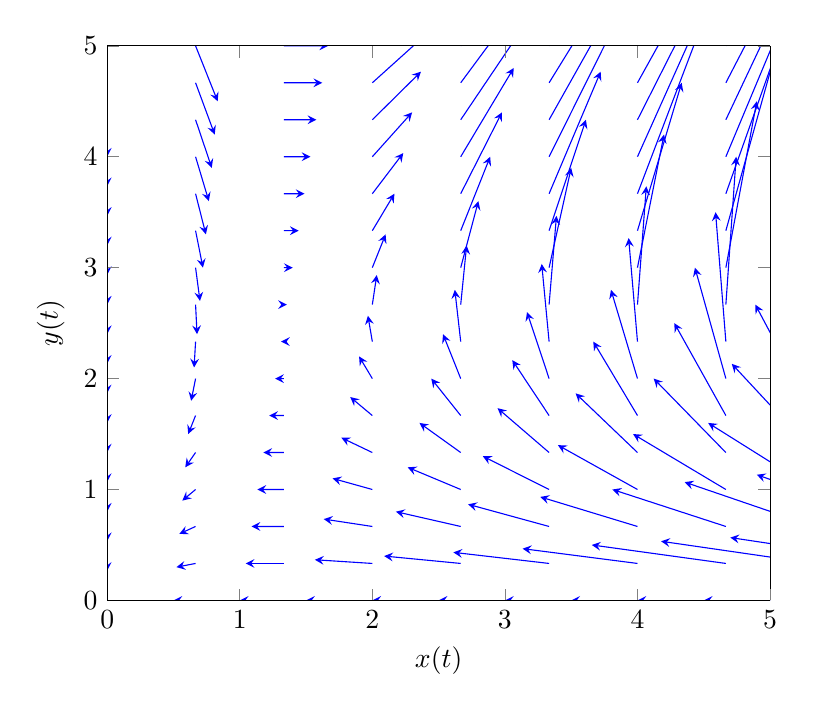
\begin{tikzpicture}
		\begin{axis}
			[
			view = {0}{90},
			domain = 0:10,
			y domain = 0:5,
			xlabel = \(x(t)\),
			ylabel = \(y(t)\),
			xmin = 0, xmax = 5,
			ymin = 0, ymax = 5,
			width = 10cm
			]
			\def\U{(-5*x)+(2*x*y)}
			\def\V{(-4*y)+(3*x*y)}
			\addplot3[blue, quiver={u=\U, v=\V, scale arrows=0.05, every arrow/.append style={-stealth}}, samples=16] (x,y,0);
		\end{axis}
	\end{tikzpicture}\\
	Figure 1: Phase Plane for \hyperref[sys]{System (A)}\label{fig:1}
\end{center}


As a corollary of this analysis, we find that for $y=\frac{5}{2}$, $\frac{\mathrm{d}x}{\mathrm{d}t} =0$, and thus our solutions for $y=\frac{5}{2}$ will only be nonzero in $x$. Specifically,
\[
	\frac{\mathrm{d}y}{\mathrm{d}t} =-\frac{20}{2}+\frac{15}{2}x=\frac{5}{2}\left( 3x-4 \right) 
	\]
for $y=\frac{5}{2}$. Notice that $\frac{\mathrm{d}y}{\mathrm{d}t} >0$ for $x>\frac{4}{3}$, and similarly $\frac{\mathrm{d}y}{\mathrm{d}t} <0$ for $x<\frac{4}{3}$.

Similarly, if we set $\frac{\mathrm{d}y}{\mathrm{d}t} =0$, we have $x=\frac{4}{3}$. Thus, for any solution with $x=\frac{4}{3}$, our solution will be zero in $y$, and we only have to analyze its behavior in $x$. Plugging this into $\frac{\mathrm{d}x}{\mathrm{d}t} $ yields
\[
	\frac{\mathrm{d}x}{\mathrm{d}t} =-\frac{20}{3}+\frac{8}{3}y=\frac{4}{3}\left( 2y-5 \right) 
.\]
Notice that for $y<\frac{5}{2}$, we have $\frac{\mathrm{d}x}{\mathrm{d}t} <0$, and likewise for $y>\frac{5}{2}$, we have $\frac{\mathrm{d}x}{\mathrm{d}t} >0$. These solutions are all included in \hyperref[fig:4]{figure 4} later.

\subsection{System (B)}
The analysis of \hyperref[sys]{system (B)} is slightly more involved, so we will gloss over the simple calculations and focus on the more indepth ones. First, we will identify system behavior for either $x_0=0$ or $y_0=0$. Notice for $x_0=0$, we have $\frac{\mathrm{d}x}{\mathrm{d}t} =0$ and $\frac{\mathrm{d}y}{\mathrm{d}t} =y(5-2y)$. It follows that $(0,0)$ and $(0,5 / 2)$ are equilibrium points of the system. Additionally, since $\frac{\mathrm{d}y}{\mathrm{d}t} <0$ for $y\in(0,5 / 2)$, and since $\frac{\mathrm{d}y}{\mathrm{d}t} $ is continuous in $y$ and has two distinct roots, by the fundamental theorem of algebra and the mean value theorem $\frac{\mathrm{d}y}{\mathrm{d}t} >0$ for $y>5 / 2$.

Now let $y_0=0$, and observe $\frac{\mathrm{d}y}{\mathrm{d}t} =0$ and $\frac{\mathrm{d}x}{\mathrm{d}t} =x(6-x)$. This gives us equilibria at $(0,0)$ and $(6,0)$, and similarly, $\frac{\mathrm{d}x}{\mathrm{d}t} <0$ for $x\in(0,6)$ and $\frac{\mathrm{d}x}{\mathrm{d}t} >0$ for $x>6$.

Notice that for $\frac{\mathrm{d}y}{\mathrm{d}t} =0$, we have $x=\frac{5-2y}{2}$, and for $\frac{\mathrm{d}x}{\mathrm{d}t} =0$, we have $y=\frac{6-x}{4}$. These linear functions correspond to lines where the vector field is compeltely horizontal and completely vertical, respectively. Also notice that if we find the intersection of these lines by set ting
\[
	\frac{6-x}{4}=\frac{5-2y}{2}
,\]
we find a new equilibrium point, $(x,y)=\left( \frac{4}{3},\frac{7}{6} \right) $. We have found that the set of all equilibrium points is $\left\{ (0,0),(0,5 / 2),(6,0),(4 / 3,7 / 6) \right\} $.

\setcounter{figure}{1}
\begin{figure}[ht]
	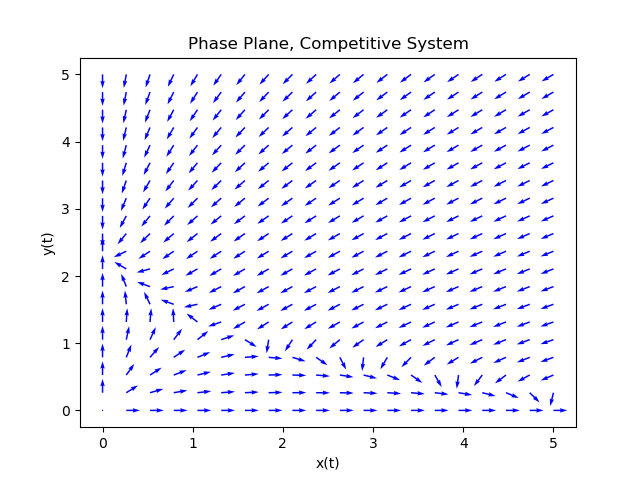
\includegraphics[scale=0.75]{Project/Phase Plane, Competitive System.png}
	\centering
	\caption{Phase Plane for \hyperref[sys]{System (B)}}\label{fig:2}
	\centering
\end{figure}
\section{Classification of all Solutions}\label{sec:3}
Further analysis with Euler's Method allows us to approximate multiple solution curves. \hyperref[fig:4]{Figure 4} depicts the approximated solution curves for a variety of initial values, along with all equilibrium points of the system, and all lines along which either $\frac{\mathrm{d}x}{\mathrm{d}t} $ or $\frac{\mathrm{d}y}{\mathrm{d}t} $ equal 0, for which $x,y\neq 0$. Red dots indicate an initial condition, and blue dots indicate an equilibria. Red lines indicate a line along which $\frac{dx}{dt}=0$, and green lines indicate a line along which $\frac{dy}{dt}=0$. All other lines are solution curves.
\begin{figure}[ht]
	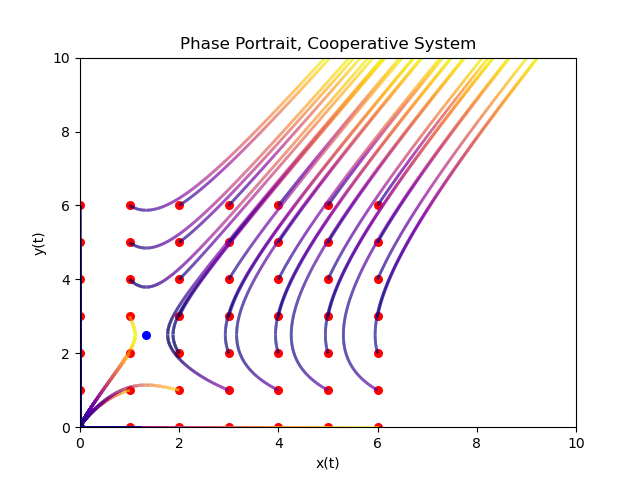
\includegraphics[scale=0.5]{Project/Phase Portrait, Cooperative System.png}
	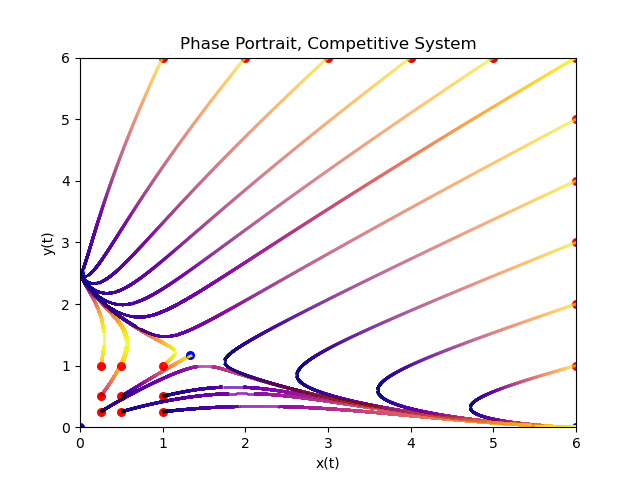
\includegraphics[scale=0.5]{Project/Phase Portrait, Competitive System.png}
	\centering
	\caption{Phase Portraits for Systems (A) and (B)}
\end{figure}
\subsection{System A}
We will begin by analyzing the equilibrium point behavior. We saw already in \hyperref[sec:2a]{section 2.1} that the equilibrium point $\left( 0,0 \right) $ behaved as a sink. However, the other equilibrium point $(4 /3, 5 / 2)$ behaves as a sort of saddle point. Solutions do not necessarily approach it, nor do they diverge from it. However, using figures \hyperref[fig:1]{1} and \hyperref[fig:3]{3}, we observe a few things about this point.

There appear to be two bounding functions, one a quadratic of the form $x=ay^2$ on the right, and another quadratic $x=-by^2$ on the left, as seen in \hyperref[fig:4]{figure 4} . However, the case is more complex than this. We use an advanced method known as ``guess a function'' to guess that $x=\frac{2}{5}\left(y-\frac{5}{2}\right)^2+\frac{4}{3}$ is this function, or is at least close to it. This shows us that although this may be the case for $x<4 /3$, for values above the equilibrium point there appears to be a linear bounding function,
\begin{figure}[ht]
	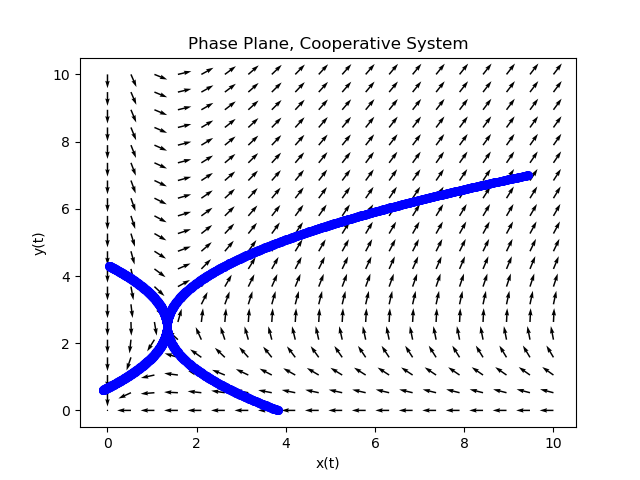
\includegraphics[scale=0.7]{Project/Phase Plane, Cooperative System.png}
	\centering
	\caption{Phase Plane for System (A) with Quadratics}\label{fig:4}
\end{figure}
which we believe is simply the line from $(0,0)$ to the equilibrium point. However, this bounding is of minor importance, since all points above the lower section of the quadratic appear to diverge. Similarly, the solutions appear to be bounded above by the same quadratic but reflected, and below the equilibrium point we claim they are subject to this same diagonal line. To summarize, we believe the following:
\begin{enumerate}
	\item For initial conditions $(x_0,y_0)$ with $x>4 /3$ and $x < 2 /5(y-5 /2)^2 +4 /3$, then $x,y\to 0$ as $t\to \infty$.
	\item For initial conditions $(x_0,y_0)$ with $x<4 /3$ and $x < 2 /5(y-5 /2)^2 +4 /3$, then $x,y\to 0$ as $t\to \infty$.
	\item For all other initial conditions, $x,y\to \infty$ as $t\to \infty$.
\end{enumerate}
Although we are not confident on the exact formulation of the bounding functions, as the $2 /5$ value was simply a guess and the other values come from the vertex being the equilibria, we believe it is at least some function of this form. Furthermore, we will note that this behavior is induced due to the functions we found where $\frac{\mathrm{d}y}{\mathrm{d}t} $ or $\frac{\mathrm{d}x}{\mathrm{d}t} =0$. These lines where the derivative is either horizontal or vertical indicate ``points of no return''. If a function crosses this line, then both $\frac{\mathrm{d}x}{\mathrm{d}t} $ and $\frac{\mathrm{d}y}{\mathrm{d}t} $ will remain positive for all $t$. In order for a function to collapse, it must reach a point wherein both of its derivatives are negative, at which point it collapses to the origin. Unfortunately, we were unable to use this fact to identify the precise equations that bounded the solutions, and more research may be necessary.

We will remark further on the line from the origin to the fixed point. Using this given information, we conjecture that
\[
	y=\frac{15}{8}x
\]
may be a straight-line solution to the system, Since the vector field tends to converge to a slope similar to this, and this line appears to have similar properties below the equilibrium point. However, this does not appear to be the case. Although solutions appear to converge to this straight line, it does not solve the system.

Finally, we will note briefly that all solutions along the $x$- and $y$-axes are purely horizotal or vertical,  respectively, and such, no function starting on the axes can leave the axes, and by Picard's theorem, no function not starting on the axes can every touch one of the axes. It follows that any solution with initial condition $x_0,y_0\in\mathbb{R}^+$ must remain in $\mathbb{R}^+$ for all $t$.

We conclude by characterizing the behavior of the populations modeled by this system. We noted that for initial conditions sufficiently small, the solutions would always collapse to the origin as $t\to \infty$. This implies that this system is not only cooperative, but rather dependent on the other population. If both populations are sufficiently small, survival is not possible. However, we also noticed that most reasonable population sizes would blow up to $\infty$, since there is no competition in this system. Although this is not realistic for real life, since there are finite resources and there would be some upper bounding behavior on a more realistic system, this can at least model short term cooperative systems, since they would exhibit similar behavior given no opposition and initially plentiful resources. We also note that since $\left( \frac{\mathrm{d}x}{\mathrm{d}t},\frac{\mathrm{d}y}{\mathrm{d}t}   \right) $ tends to approach $\left( 8,15 \right) $ in the case that the solutions blow up, we note that population $y$ tends to grow faster than population $x$.
\subsection{System (B)}
Using figures \hyperref[fig:2]{2} and \hyperref[fig:3]{3}, we notice that the equilibrium point $(0,0)$ is a source, $(0,6)$ and $(0,5/2)$ are sinks, and $(4 /3,7 /6)$ is a sort of saddle point.

We note that similarly with system (A), the system's behavior is bounded based on it's initial condition. By the same logic as previously, since the derivative is purely horizontal on the $x$-axis and vertical on the $y$-axis, any strictly positive initial condition is confined to positive values for all $t$. However, there appears to be a line of stability that all solutions inevitably approach, which looks like a quadratic which passes through $(6,0)$, $(0, 5/2)$, and $(4 /3,7 /6)$. However, the unique quadratic that passes through these points also goes into the negatives, which our line of stability clearly does not.

However, even without knowing the precise function, we can still describe the behavior around it. All solutions rapidly approach the line fairly linearly, at which point they converge fairly quickly to one of the sinks. If a point starts below the bounding function, then it will approach the bound from below, whereas if it starts from above, it will approach from above. There appears to be no case where the solution blows up to infinity.

We conclude by characterizing this analysis in the context of competitive populations. It appears that if any one species, or perhaps both species, are of populations that are too large, then the over-competition inevitably collapses them to a meta-stable state, which we would call the bounding function. Similarly, if the species' populations are sufficiently low, then competition is rare enough to fascilitate growth towards the meta-stable state. However, once populations reach meta-stability, they continue to evolve along the bounding function, eventually reaching a fully stable population where one species has gone extinct from competition, and the other lives at a stable population. The competitoin appears to provide no real benefit to either species, unlike a predator-prey model.
\bibliographystyle{amsplain}
\bibliography{refs.bib}
\appendix
\section{Code}
Figure 1 was done directly in TikZ using pfgplots and the quiver library, while all other figures were done using python using matplotlib, due to python making it easier to normalize vector lengths while accounting for dividing by zero errors, and the gradient effect in figure 4 would be difficult to replicate in a LaTeX only soltuion. I included that effect because I thought it was a fairly nice indicator of which direction a function is evolving in. Unfortunately I only found a way to get it to work in the direction of increasing $x$, rather than increasing $t$, since I did not fully understand ChatGPT's code. And because this needs to be stated: I only used ChatGPT and internet sources for plotting. I wrote all the numerical code myself. I've set the remainder of my document to single-line spacing because it's just my code.
\singlespacing
\begin{center}
	Code 1: Euler's Method Code for the Cooperative System\footnote{The only changes made for the competitive system were changing the initial conditions and the differential equations. I have 3 functions to output a graph, and I chose which one I wanted to run by uncommenting it. I did not feel like implementing a neater solution was necessary.}
\end{center}
\begin{lstlisting}[language=Python]
#!/usr/bin/env python3

import matplotlib.pyplot as plt
import os.path
import time
import matplotlib.cm as cm
import numpy as np
from matplotlib.collections import LineCollection
from matplotlib.colors import Normalize

# initial conditions
colormap = "plasma"
t_0 = 0
t_step = 0.0001
t_f = 3
x_inits = []
y_inits = []
for i in range(7):
    for j in range(7):
        x_inits.append(i)
        y_inits.append(j)
equilibria = [
        [0,4/3],
        [0,5/2]
]

# directory where I saved project files
project_dir = os.path.expanduser("~/Documents/University/bachelor_2/Semester_1/Honors_Differential_Equations/Homework/Project")

# differential equations
def diffeqX(x,y):
    return (-5 * x) + (2 * x * y)
def diffeqY(x,y):
    return (-4 * y) + (3 * x * y)

# runs the center difference euler's method because it was suprisingly the easiest to copy from my previous code
# returns the next x or y value depending on function call
def centered_eulerX(x_k, y_k, x_kk, delta_t):
    return x_kk + (diffeqX(x_k, y_k) * 2 * delta_t)
def centered_eulerY(x_k, y_k, y_kk, delta_t):
    return y_kk + (diffeqY(x_k, y_k) * 2 * delta_t)

# generates a list of t values
# returns the list
def gen_t_vals(t_final, delta_t, t_init):
    temp = [t_init]
    t = t_init
    while t <= t_final:
        temp.append(t)
        t += delta_t
    return temp

# runs euler's method
# returns 2 lists of approximated values
def run_euler(x_0, y_0, t_list, t_step):
    x_list = [x_0, x_0 + (t_step * diffeqX(x_0,y_0))]
    y_list = [y_0, y_0 + (t_step * diffeqY(x_0,y_0))]
    for t in t_list[2:]:
        x_list.append(centered_eulerX(x_list[len(x_list) - 1], y_list[len(y_list) - 1], x_list[len(x_list) - 2], t_step))
        y_list.append(centered_eulerY(x_list[len(x_list) - 1], y_list[len(y_list) - 1], y_list[len(y_list) - 2], t_step))
        if x_list[len(x_list)-1] > 10 or y_list[len(y_list)-1] > 10:
            break
    return x_list, y_list

# plots all approximated solutions, initial conditions, equilibria, and the vector field F=(dx,dy)
def plotting(tensorX, tensorY, t_list):
    for i in range(len(tensorX)):
        # chatgpt code for gradient lines
        # im not sure what reshape is
        points = np.array([tensorX[i], tensorY[i]]).T.reshape(-1, 1, 2)
        # ?????? what is this code
        segments = np.concatenate([points[:-1], points[1:]], axis=1)

        norm = Normalize(vmin=min(tensorX[i]), vmax=max(tensorX[i]))
        lc = LineCollection(segments, cmap=colormap, norm=norm)
        lc.set_array(tensorX[i])
        lc.set_linewidth(2)

        plt.gca().add_collection(lc)

    plt.xlim(0,10)
    plt.ylim(0,10)
    plt.scatter(x_inits, y_inits, color="red", label="Initial values", s=30)
    plt.scatter(equilibria[0], equilibria[1], label="Equilibrium points", color="blue", s=30)

    # generates a vector field on top of the lines
    x_lin = np.linspace(0,10,20)
    y_lin = np.linspace(0,10,20)
    X, Y = np.meshgrid(x_lin, y_lin)
    U = diffeqX(X, Y)
    V = diffeqY(X, Y)

    magnitude = np.sqrt(U**2 + V**2)
    U_norm = np.where(magnitude == 0, 0, U / magnitude)
    V_norm = np.where(magnitude == 0, 0, V / magnitude)
    plt.quiver(X, Y, U_norm, V_norm, angles="xy")

    plt.show()

# plots only the solutions, equilibria, and initial conditions
def plot_lines(tensorX, tensorY, t_list):
    for i in range(len(tensorX)):
        # chatgpt code for gradient lines
        # im not sure what reshape is
        points = np.array([tensorX[i], tensorY[i]]).T.reshape(-1, 1, 2)
        # ??????
        segments = np.concatenate([points[:-1], points[1:]], axis=1)

        norm = Normalize(vmin=min(tensorX[i]), vmax=max(tensorX[i]))
        lc = LineCollection(segments, cmap=colormap, norm=norm)
        lc.set_array(tensorX[i])
        lc.set_linewidth(2)

        plt.gca().add_collection(lc)
    plt.xlim(0,10)
    plt.ylim(0,10)
    plt.scatter(x_inits, y_inits, color="red", label="Initial values", s=30)
    plt.scatter(equilibria[0], equilibria[1], label="Equilibrium points", color="blue", s=30)
    #plt.colorbar(lc, label="value along the line")

    plt.xlabel("x(t)")
    plt.ylabel("y(t)")
    plt.title("Phase Portrait, Cooperative System")
    plt.savefig(os.path.join(project_dir,"Phase Portrait, Cooperative System.png"))
    plt.show()

# plots only the vector field
def vector_field():
    x_lin = np.linspace(0,10,20)
    y_lin = np.linspace(0,10,20)
    X, Y = np.meshgrid(x_lin, y_lin)
    U = diffeqX(X, Y)
    V = diffeqY(X, Y)

    magnitude = np.sqrt(U**2 + V**2)
    U_norm = np.where(magnitude == 0, 0, U / magnitude)
    V_norm = np.where(magnitude == 0, 0, V / magnitude)
    plt.quiver(X, Y, U_norm, V_norm, angles="xy")
    plt.xlabel("x(t)")
    plt.ylabel("y(t)")
    plt.title("Phase Plane, Cooperative System")
    plt.savefig(os.path.join(project_dir,"Phase Plane, Cooperative System.png"))
    plt.show()

def main():
    # check if inital conditions were entered correctly
    if len(y_inits) != len(x_inits):
        raise ValueError("Different numbers of x and y initial conditions.")

    # we need to store lists of x and y
    x_vals = []
    y_vals = []
    start = time.time()
    t_vals = gen_t_vals(t_f, t_step, t_0)
    time1 = time.time()
    print(f"t values generated in {time1 - start}")
    for i in range(len(y_inits)):
        tempX, tempY = run_euler(x_inits[i], y_inits[i], t_vals, t_step)
        x_vals.append(tempX)
        y_vals.append(tempY)
    print(f"euler ran in {time.time() - time1}")

    #plotting(x_vals, y_vals, t_vals)
    plot_lines(x_vals, y_vals, t_vals)
    #vector_field()

if __name__ == "__main__":
    main()

\end{lstlisting}
\newpage
\section{Figure 3}
\begin{figure}[ht]
	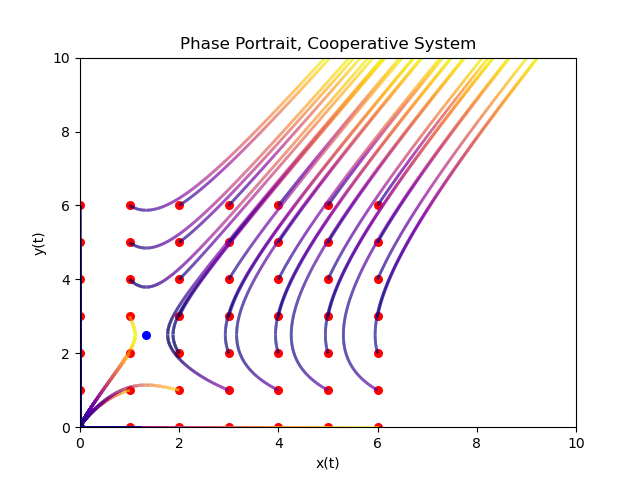
\includegraphics{Project/Phase Portrait, Cooperative System.png}
	\centering
\end{figure}
\begin{figure}[ht]
	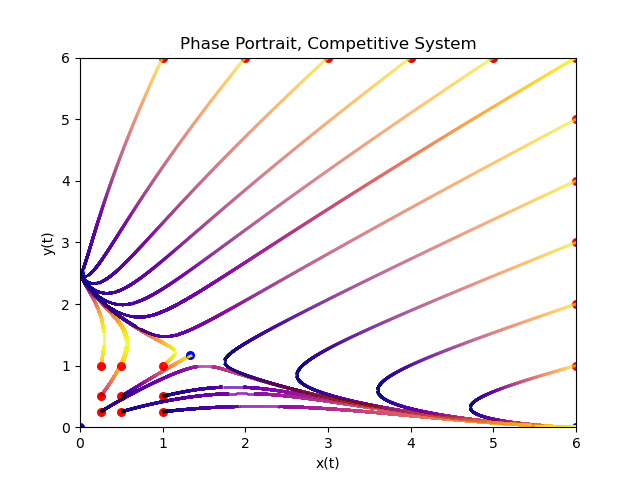
\includegraphics{Project/Phase Portrait, Competitive System.png}
	\centering
\end{figure}
\end{document}
